% Generated by book/tools/notebook_to_tex.py. Do not edit by hand.

\chapter[BERT 다중 라벨 분류 (Multi-label \& Per-label BCE)]{BERT 다중 라벨 분류 (Multi-label \& Per-label BCE)}

\label{ch:13}

\markboth{BERT 다중 라벨 분류 (Multi-label \& Per-label BCE)}{BERT 다중 라벨 분류 (Multi-label \& Per-label BCE)}

\chaptermeta{13_bert_multilabel/13_bert_multilabel.ipynb}{https://colab.research.google.com/github/yoon-gu/neuqes-101/blob/master/13_bert_multilabel/13_bert_multilabel.ipynb}{Yelp 항목 합성 라벨을 BERT의 라벨별 sigmoid와 BCE로 학습}



\index{1BERT multi label classification@BERT multi-label classification}

\index{1multi label classification@multi-label classification}

\index{1BCEWithLogitsLoss@BCEWithLogitsLoss}

\index{1num labels 5@num\_labels=5}

\index{1multi label classification@multi\_label\_classification}

\index{1multi hot label@multi-hot label}

\index{1per label sigmoid@per-label sigmoid}

\index{1hamming loss@hamming\_loss}

\index{1micro F1@micro F1}

\index{1macro F1@macro F1}

\index{1OneVsRestClassifier@OneVsRestClassifier}

\index{1label co occurrence@label co-occurrence}

\index{0다중 라벨 분류@다중 라벨 분류}

\index{0멀티핫@멀티핫}

\index{0라벨별 시그모이드@라벨별 시그모이드}

\index{0라벨별 BCE@라벨별 BCE}

\index{0공동 활성@공동 활성}

\index{0항목 라벨@항목 라벨}

\index{0해밍 손실@해밍 손실}

\index{1AutoModelForSequenceClassification@AutoModelForSequenceClassification}

\index{1problem type multi label classification@problem\_type="multi\_label\_classification"}

\index{1roc auc score@roc\_auc\_score}

\index{1seaborn FacetGrid@seaborn.FacetGrid}

\index{1co occurrence matrix@co-occurrence matrix}

\index{1conditional probability@conditional probability}

\index{1binary relevance@binary relevance}

\index{0항목 키워드@항목 키워드}

\index{0조건부 확률@조건부 확률}

\index{0라벨 공기@라벨 공기}

\index{0이진 관련성@이진 관련성}



\section{변화추적표}

\begin{booktable}{13장 변화추적표}{tab:ch13-01}
\begin{adjustbox}{max width=\textwidth}
\begin{tabular}{@{}lllllll@{}}
\toprule
Ch & 모델 & 토크나이저 & 데이터 & Output Head & Activation & Loss \\
\midrule

6 & \inlinecode{OneVsRestClassifier(LogisticRegression())} & \inlinecode{TfidfVectorizer()} & Yelp + 항목 키워드 합성 & (5차원) & sigmoid (각각) & \inlinecode{BCEWithLogitsLoss} per-label \\
10 & DistilBERT 파인튜닝 & \inlinecode{AutoTokenizer.from\_pretrained(...)} & Yelp 이진화 & \inlinecode{Linear(H,\ 1)} & sigmoid & \inlinecode{BCEWithLogitsLoss} \\
12 & DistilBERT 파인튜닝 & 같음 & Yelp 5클래스 & \inlinecode{Linear(H,\ 5)} & softmax & \inlinecode{CrossEntropyLoss} \\
\textbf{13 \(\leftarrow\) 여기} & DistilBERT 파인튜닝 & 같음 & \textbf{Yelp + 항목 키워드 합성} & \textbf{\inlinecode{Linear(H,\ 5)}} & \textbf{sigmoid (per-label)} & \textbf{\inlinecode{BCEWithLogitsLoss} (per-label)} \\
14 (다음) & DistilBERT 파인튜닝 & 같음 & Yelp + 항목 + 별점 보조 & \inlinecode{Linear(H,\ 5)} 메인 + \inlinecode{Linear(H,\ 1)} 보조 & sigmoid + 없음 & \texttt{BCE(per-label)\ +\ \$\textbackslash{}lambda\$·MSE} \\
\bottomrule
\end{tabular}
\end{adjustbox}
\end{booktable}

전체 장 표는 \href{https://github.com/yoon-gu/neuqes-101\#챕터별-변화추적표}{루트 README.md}를 참고하세요.



\section{변경점: \ref{ch:12}장 대비}

\begin{booktable}{13장 변경점 요약}{tab:ch13-02}
\begin{adjustbox}{max width=\textwidth}
\begin{tabular}{@{}lll@{}}
\toprule
축 & \ref{ch:12}장 (multi-class) & \ref{ch:13}장 (multi-label) \\
\midrule

\textbf{Task} & 5클래스 \emph{single-label} (서로 배타적) & \textbf{5라벨 \emph{multi-label}} (동시 활성 가능) \(\leftarrow\) 본질적 변화 \\
\inlinecode{num\_labels} & 5 & \textbf{5} (그대로!) \\
\inlinecode{problem\_type} & \inlinecode{"single\_label\_classification"} & \textbf{\inlinecode{"multi\_label\_classification"}} \(\leftarrow\) BCE 자동 매핑 \\
Activation & softmax (합=1 강제) & \textbf{per-label sigmoid} (각각 독립 0-1) \\
Loss & \inlinecode{CrossEntropyLoss} & \textbf{\inlinecode{BCEWithLogitsLoss}} per-label \\
라벨 형식 & int 스칼라 (0-4) & \textbf{multi-hot float \texttt{{[}1,\ 0,\ 1,\ 0,\ 1{]}}} \\
모델 출력 의미 & logits{[}k{]} = 클래스 k의 \emph{상대적} 점수 & logits{[}k{]} = 라벨 k의 \emph{독립적} 활성 점수 \\
평가 metric & accuracy + macro F1 + AUC OvR & per-label precision/recall/F1 + micro/macro F1 + per-label AUC \\
\bottomrule
\end{tabular}
\end{adjustbox}
\end{booktable}

\begin{quote}
\textbf{결정적 인사이트}: 모델 \emph{아키텍처는 동일} --- \inlinecode{Linear(H,\ 5)} 헤드. 변하는 건 \emph{해석} 과 그에 따른 loss/activation입니다. 같은 5차원 출력을 \emph{softmax로 모아서 한 클래스 고르기} 와 \emph{5개 sigmoid로 각자 0/1 결정하기} 두 가지로 다르게 쓰는 것.
\end{quote}

\subsection{왜 multi-label은 softmax로 풀 수 없는가}

softmax는 출력의 \emph{합 = 1} 을 강제합니다 (\(\sum_k \mathrm{softmax}(z)_k = 1\)). 이는 \emph{서로 배타적} 클래스에 자연스럽지만 multi-label과 충돌합니다.

리뷰가 “food=1 (음식 언급) 그리고 service=1 (서비스 언급)” 일 때:

\begin{itemize}
\tightlist
\item
  \textbf{softmax 모델은 표현 불가}: P(food)=0.9 면 나머지 4 라벨 합이 0.1 로 강제 \(\to\) \textquotesingle service=0.85 동시 활성\textquotesingle{} 이 \emph{수학적으로 불가능}.
\item
  \textbf{per-label sigmoid 모델은 표현 가능}: 각 라벨이 독립이라 P(food)=0.9 와 P(service)=0.85 가 동시에 자연스러움.
\end{itemize}

즉 task가 \emph{진짜 multi-label} 이라면 loss/activation 선택이 강제됩니다 (\ref{ch:06}장에서 본 동일한 논리, BERT로 옮겨옴).



\section{\texorpdfstring{손실 노트}{손실 노트}}

K개 라벨 각각에 \emph{독립적} BCE를 적용한 뒤 평균:

\begin{equation}
\label{eq:ch13-01}
L = \frac{1}{N \cdot K}\sum_{i=1}^{N}\sum_{k=1}^{K}\left[ y_{i,k} \log \sigma(z_{i,k}) + (1-y_{i,k}) \log(1-\sigma(z_{i,k})) \right]
\end{equation}

식~\eqref{eq:ch13-01}은 이 절에서 사용하는 핵심 관계를 정리한 것입니다.

각 \(z_{i,k}\) 는 \emph{독립 logit} --- 라벨 k가 \emph{얼마나 활성될지} 의 점수, 다른 라벨과 무관. PyTorch \inlinecode{BCEWithLogitsLoss} 가 5개 위치를 한 번에 처리하지만 수식적으론 K개의 binary BCE 평균.

\textbf{숫자로 감 잡기 (K=5, 정답 multi-hot \(\mathbf{y} = [1, 0, 1, 0, 1]\))} --- logits 별 손실 분해:

\begin{booktable}{13장 손실 노트 표}{tab:ch13-03}
\begin{adjustbox}{max width=\textwidth}
\begin{tabular}{@{}lllll@{}}
\toprule
라벨 & \(y_k\) & logit \(z_k\) & \(\sigma(z_k)\) & 정답일 때 손실 \\
\midrule

food & 1 & 3.0 & 0.953 & \(-\log 0.953 = 0.048\) \\
service & 0 & -2.0 & 0.119 & \(-\log(1-0.119) = 0.127\) \\
price & 1 & 0.5 & 0.622 & \(-\log 0.622 = 0.474\) \\
ambiance & 0 & 1.5 & 0.818 & \(-\log(1-0.818) = 1.704\) \(\leftarrow\) 자신 있게 틀림 \\
location & 1 & -0.5 & 0.378 & \(-\log 0.378 = 0.974\) \\
\bottomrule
\end{tabular}
\end{adjustbox}
\end{booktable}

평균 loss = \((0.048 + 0.127 + 0.474 + 1.704 + 0.974) / 5 \approx 0.665\).

\textbf{핵심 직관 --- 라벨 사이엔 직접 신호가 없음}: BCE per-label은 라벨 k의 logit이 라벨 j의 정답에서 \emph{직접} 학습 신호를 받지 않습니다. 모델이 라벨 간 상관을 학습하는 건 \emph{공유 BERT 본체} (모든 라벨이 같은 768-dim CLS 표현에서 옴) 덕분이지 loss 자체에는 라벨 간 결합 항이 없습니다. 이 점이 multi-class softmax와 결정적 차이.



\section{토크나이저 노트}

\ref{ch:12}장과 동일 --- \inlinecode{distilbert-base-uncased} WordPiece, \inlinecode{max\_length=128}. 토크나이저는 라벨 \emph{형식} 에 무관하므로 single-label 이든 multi-label 이든 변화 없음.

\begin{previewBox}{미리보기}
\textbf{다음 장(\ref{ch:14}장)}: 토크나이저 그대로. 변하는 건 \emph{모델에 보조 헤드} 가 추가되고 \emph{loss에 보조 항} 이 가중합으로 더해지는 점.
\end{previewBox}



\Needspace{5\baselineskip}
\begin{lstlisting}
!pip install -q transformers datasets
\end{lstlisting}

\begin{codeRead}
\textbf{1행}의 \inlinecode{!pip install -q transform...}에서는 Colab 실행에 필요한 패키지를 설치합니다.
\end{codeRead}



\Needspace{11\baselineskip}
\begin{lstlisting}
import warnings
warnings.filterwarnings("ignore")

import re
import numpy as np
import pandas as pd
import matplotlib.pyplot as plt
import seaborn as sns
import torch
from datasets import Dataset, load_dataset
from transformers import (
    AutoTokenizer, AutoModelForSequenceClassification,
    Trainer, TrainingArguments,
)
from sklearn.metrics import (
    precision_recall_fscore_support, classification_report,
\end{lstlisting}

\noindent\emph{앞뒤 블록은 모두 필요한 라이브러리와 기본 설정을 준비하는 단계입니다. 길이를 나누어 같은 흐름을 단계별로 확인합니다.}

\Needspace{11\baselineskip}
\begin{lstlisting}[firstnumber=17]
    roc_auc_score, hamming_loss,
)

from sklearn.feature_extraction.text import TfidfVectorizer
from sklearn.linear_model import LogisticRegression
from sklearn.multiclass import OneVsRestClassifier

import matplotlib.pyplot as plt, matplotlib.font_manager as fm, subprocess, os
_fp = "/usr/share/fonts/truetype/nanum/NanumGothic.ttf"
if not os.path.exists(_fp):
    subprocess.run(
        "apt-get -qq -y install fonts-nanum",
        shell=True,
    )
fm.fontManager.addfont(_fp)
plt.rcParams["font.family"] = "NanumGothic"
\end{lstlisting}

\noindent\emph{앞 블록은 필요한 라이브러리와 기본 설정을 준비하는 단계입니다. 이어지는 블록에서는 숫자 결과를 그림으로 확인하는 단계로 넘어갑니다.}

\Needspace{11\baselineskip}
\begin{lstlisting}[firstnumber=33]
plt.rcParams["axes.unicode_minus"] = False

print(f"PyTorch:        {torch.__version__}")
print(f"CUDA available: {torch.cuda.is_available()}")
if torch.cuda.is_available():
    print(
        f"GPU:             "
        f"{torch.cuda.get_device_name(0)}"
    )
else:
    print(
        "Warning: CPU runtime — training will be very "
        "slow. Switch to T4 recommended."
    )
\end{lstlisting}

\begin{codeRead}
\inlinecode{numpy, pandas, matplotlib, PyTorch, datasets} 같은 주요 패키지를 불러옵니다.
\end{codeRead}

\noindent\textbf{출력.}
\begin{bookoutputbox}
PyTorch:        2.11.0+cu128
CUDA available: True
GPU:             Tesla T4
\end{bookoutputbox}
\par\vspace{0.9em}



\textbf{baseline VRAM}:



\Needspace{5\baselineskip}
\begin{lstlisting}
!nvidia-smi
\end{lstlisting}

\begin{codeRead}
\textbf{1행}의 \inlinecode{!nvidia-smi}에서는 앞 단계에서 만든 값을 바탕으로 다음 계산을 수행합니다.
\end{codeRead}

\noindent\textbf{출력.}
\begin{bookoutputbox}
Mon Jun 22 03:49:55 2026
NVIDIA-SMI 580.82.07 Driver Version: 580.82.07 CUDA Version: 13.0
0 Tesla T4 Off | 00000000:00:04.0 Off | 0
N/A 46C P8 11W / 70W | 3MiB / 15360MiB | 0% Default
\end{bookoutputbox}
\par\vspace{0.9em}



\section{데이터 준비}

Yelp 리뷰엔 multi-label 정답이 없습니다. \ref{ch:06}장에서처럼 5개 항목(aspect)별 키워드 사전을 만들어 텍스트에서 매칭 --- 어떤 키워드라도 등장하면 해당 항목을 1로 활성. 5차원 multi-hot 벡터가 합성됩니다.

\begin{booktable}{13장 데이터 준비 표}{tab:ch13-04}
\begin{adjustbox}{max width=\textwidth}
\begin{tabular}{@{}lll@{}}
\toprule
항목 & 의미 & 키워드 예시 \\
\midrule

\inlinecode{food} & 음식의 맛/메뉴 & food, meal, dish, taste, delicious, ... \\
\inlinecode{service} & 서비스/응대 & service, staff, waiter, friendly, rude, ... \\
\inlinecode{price} & 가격/가성비 & price, cheap, expensive, value, worth, ... \\
\inlinecode{ambiance} & 분위기/인테리어 & atmosphere, decor, music, vibe, cozy, ... \\
\inlinecode{location} & 위치/주차 & location, parking, area, neighborhood, ... \\
\bottomrule
\end{tabular}
\end{adjustbox}
\end{booktable}

\begin{quote}
\textbf{합성의 한계} --- 키워드 매칭은 \emph{언급한 항목} 만 잡고 \emph{언급한 항목이 긍정인지 부정인지} 는 알 수 없습니다. 또 \emph{키워드 없이} 항목이 표현된 경우(예: “10 minutes wait” \(\to\) service)도 놓칩니다. 이 한계는 장 끝에서 솔직히 짚습니다.
\end{quote}



\Needspace{11\baselineskip}
\begin{lstlisting}
ASPECT_KEYWORDS = {
    "food": ["food", "meal", "dish", "taste", "delicious", "flavor", "menu",
             "cuisine", "tasty", "yummy", "spicy", "sweet", "salty", "fresh"],
    "service": ["service", "staff", "waiter", "waitress", "server", "friendly",
                "rude", "attentive", "host", "helpful", "polite", "manager"],
    "price": ["price", "cheap", "expensive", "value", "worth", "cost",
              "money", "afford", "overpriced", "pricey", "deal", "bargain"],
    "ambiance": ["atmosphere", "ambiance", "decor", "music", "vibe", "cozy",
                 "noisy", "quiet", "lighting", "interior", "comfortable", "loud"],
    "location": ["location", "parking", "area", "neighborhood", "access",
                 "downtown", "convenient", "spot"],
}
ASPECTS = list(ASPECT_KEYWORDS.keys())
K = len(ASPECTS)

\end{lstlisting}

\noindent\emph{앞뒤 블록은 모두 앞에서 만든 중간 값을 다음 계산으로 넘기는 단계입니다. 길이를 나누어 같은 흐름을 단계별로 확인합니다.}

\Needspace{11\baselineskip}
\begin{lstlisting}[firstnumber=16]
def extract_aspects(text: str) -> list[float]:
    text_lower = text.lower()
    return [
        float(any(re.search(rf"\b{re.escape(kw)}\b", text_lower) for kw in keywords))
        for keywords in ASPECT_KEYWORDS.values()
    ]

print(f"K (number of aspects): {K}")
print(f"aspects: {ASPECTS}")
\end{lstlisting}

\noindent\textbf{출력.}
\begin{bookoutputbox}
K (number of aspects): 5
aspects: ['food', 'service', 'price', 'ambiance', 'location']
\end{bookoutputbox}
\par\vspace{0.9em}



\Needspace{11\baselineskip}
\begin{lstlisting}
tokenizer = AutoTokenizer.from_pretrained("distilbert-base-uncased")

ds = load_dataset("Yelp/yelp_review_full")
train_full = ds["train"].shuffle(seed=42).select(range(5000))
eval_full  = ds["test"].shuffle(seed=42).select(range(1000))

def attach_aspects(batch):
    batch["aspects"] = [extract_aspects(t) for t in batch["text"]]
    return batch

train_full = train_full.map(attach_aspects, batched=True)
eval_full  = eval_full.map(attach_aspects,  batched=True)

\end{lstlisting}

\noindent\emph{앞 블록은 데이터를 불러오고 학습에 맞는 형태로 정리하는 단계입니다. 이어지는 블록에서는 앞에서 만든 중간 값을 다음 계산으로 넘기는 단계로 넘어갑니다.}

\Needspace{11\baselineskip}
\begin{lstlisting}[firstnumber=14]
print(f"train: {len(train_full)}, eval: {len(eval_full)}")
print(f"\nFirst sample:")
print(f"  text: {train_full[0]['text'][:150]}...")
print(
    f"  aspects (multi-hot): "
    f"{train_full[0]['aspects']}"
)
print(
    f"  active aspects: "
    f"{[a for a, v in zip(ASPECTS, train_full[0]['aspects']) if v > 0]}"
)
\end{lstlisting}

\noindent\textbf{출력.}
\begin{bookoutputbox}
train: 5000, eval: 1000

First sample:
text: I stalk this truck. I've been to industrial parks where I pretend to...
  aspects (multi-hot): [0.0, 1.0, 0.0, 0.0, 1.0]
  active aspects: ['service', 'location']
\end{bookoutputbox}
\par\vspace{0.9em}



\Needspace{11\baselineskip}
\begin{lstlisting}
Y_train = np.array(train_full["aspects"])
Y_eval  = np.array(eval_full["aspects"])

print("Per-aspect activation rate (train):")
for k, aspect in enumerate(ASPECTS):
    rate = Y_train[:, k].mean()
    print(
        f"  {aspect:>9}: {rate:.1%}  ({int(Y_train[:, k].sum())} / "
        f"{len(Y_train)})"
    )

\end{lstlisting}

\noindent\emph{앞뒤 블록은 모두 앞에서 만든 중간 값을 다음 계산으로 넘기는 단계입니다. 길이를 나누어 같은 흐름을 단계별로 확인합니다.}

\Needspace{11\baselineskip}
\begin{lstlisting}[firstnumber=12]
n_active = Y_train.sum(axis=1)
print(
    f"\nMean active labels per sample: "
    f"{n_active.mean():.2f}"
)
print(f"Active label distribution (train):")
for n in range(K + 1):
    cnt = (n_active == n).sum()
    print(
        f"  {n} labels active: {cnt} samples ("
        f"{cnt/len(Y_train):.1%})"
    )
\end{lstlisting}

\noindent\textbf{출력.}
\begin{bookoutputbox}
Per-aspect activation rate (train):
       food: 55.6%  (2778 / 5000)
    service: 49.6%  (2480 / 5000)
      price: 29.4%  (1472 / 5000)
   ambiance: 18.1%  (905 / 5000)
   location: 21.9%  (1095 / 5000)

Mean active labels per sample: 1.75
Active label distribution (train):
  0 labels active: 741 samples (14.8%)
  1 labels active: 1464 samples (29.3%)
  2 labels active: 1506 samples (30.1%)
  3 labels active: 957 samples (19.1%)
  4 labels active: 277 samples (5.5%)
  5 labels active: 55 samples (1.1%)
\end{bookoutputbox}
\par\vspace{0.9em}



\textbf{\ref{ch:12}장과의 한 줄 차이}: \texttt{out{[}“labels”{]}\ =\ {[}int(l)\ for\ l\ in\ batch{[}“label”{]}{]}} \(\to\) \texttt{out{[}“labels”{]}\ =\ {[}list(map(float,\ a))\ for\ a\ in\ batch{[}“aspects”{]}{]}}. 라벨이 \emph{int 스칼라} 가 아니라 \emph{길이 5 multi-hot float 벡터}. 이 형식 + \inlinecode{problem\_type="multi\_label\_classification"} 두 가지가 BCE per-label 자동 매핑의 트리거.



\Needspace{11\baselineskip}
\begin{lstlisting}
def tokenize_fn(batch):
    out = tokenizer(
        batch["text"],
        truncation=True,
        max_length=128,
    )

    out["labels"] = [list(map(float, a)) for a in batch["aspects"]]
    return out

train_tok = train_full.map(tokenize_fn, batched=True).remove_columns(["text", "label", "aspects"])
eval_tok  = eval_full.map(tokenize_fn,  batched=True).remove_columns(["text", "label", "aspects"])

\end{lstlisting}

\noindent\emph{앞 블록은 텍스트를 모델 입력 텐서로 바꾸는 단계입니다. 이어지는 블록에서는 앞에서 만든 중간 값을 다음 계산으로 넘기는 단계로 넘어갑니다.}

\Needspace{7\baselineskip}
\begin{lstlisting}[firstnumber=14]
print(train_tok)
print(
    f"\nFirst sample label: "
    f"{train_tok[0]['labels']}  (length-5 multi-hot float vector)"
)
\end{lstlisting}

\noindent\textbf{출력.}
\begin{bookoutputbox}
Dataset({
    features: ['input_ids', 'token_type_ids', 'attention_mask', 'labels'],
    num_rows: 5000
})

First sample label: [0.0, 1.0, 0.0, 0.0, 1.0] (length-5 multi-hot float vec...
\end{bookoutputbox}
\par\vspace{0.9em}



\section{\texorpdfstring{모델 로드}{모델 로드}}

\ref{ch:12}장과 \emph{모델 아키텍처는 동일} (\inlinecode{Linear(H,\ 5)} 분류 헤드). 변하는 한 가지 --- \inlinecode{problem\_type="multi\_label\_classification"} --- 가 자동 매핑되는 loss를 BCE per-label 로 바꿉니다.



\Needspace{11\baselineskip}
\begin{lstlisting}
model = AutoModelForSequenceClassification.from_pretrained(
    "distilbert-base-uncased",
    num_labels=K,
    problem_type="multi_label_classification",
    id2label={i: a for i, a in enumerate(ASPECTS)},
    label2id={a: i for i, a in enumerate(ASPECTS)},
)

def param_summary(m):
    total     = sum(p.numel() for p in m.parameters())
    trainable = sum(p.numel() for p in m.parameters() if p.requires_grad)
    return total, trainable

\end{lstlisting}

\noindent\emph{앞뒤 블록은 모두 앞에서 만든 중간 값을 다음 계산으로 넘기는 단계입니다. 길이를 나누어 같은 흐름을 단계별로 확인합니다.}

\Needspace{11\baselineskip}
\begin{lstlisting}[firstnumber=14]
total, trainable = param_summary(model)
print(
    f"Parameters:           {total:>13,}  ("
    f"{total/1e6:.1f} M)"
)
print(
    f"Trainable parameters: {trainable:>13,}  ("
    f"{trainable/total:.1%})"
)
print(f"Classifier:           {model.classifier}")
print(
    f"problem_type:         "
    f"{model.config.problem_type}"
)
print(f"id2label:             {model.config.id2label}")
\end{lstlisting}

\noindent\textbf{출력.}
\begin{bookoutputbox}
Key                     | Status     | 
------------------------+------------+-
classifier.weight       | MISSING    | 
classifier.bias         | MISSING    | 
pre_classifier.bias     | MISSING    | 
pre_classifier.weight   | MISSING    | 

- MISSING: those params were newly initialized because missing from the che...
Parameters:              66,957,317  (67.0 M)
Trainable parameters:    66,957,317  (100.0%)
Classifier:           Linear(in_features=768, out_features=5, bias=True)
problem_type:         multi_label_classification
id2label: {0: 'food', 1: 'service', 2: 'price', 3: 'ambiance', 4: 'location'}
\end{bookoutputbox}
\par\vspace{0.9em}



\textbf{\ref{ch:12}장과 파라미터 수가 \emph{완전히 동일}} --- 차이는 \inlinecode{problem\_type} 한 줄뿐. 같은 모델이 \emph{어떻게 해석되고 어떤 loss로 학습되는가} 만 바뀝니다.



\Needspace{5\baselineskip}
\begin{lstlisting}
!nvidia-smi
\end{lstlisting}

\noindent\textbf{출력.}
\begin{bookoutputbox}
Mon Jun 22 03:50:22 2026
NVIDIA-SMI 580.82.07 Driver Version: 580.82.07 CUDA Version: 13.0
0 Tesla T4 Off | 00000000:00:04.0 Off | 0
N/A 47C P8 14W / 70W | 3MiB / 15360MiB | 0% Default
\end{bookoutputbox}
\par\vspace{0.9em}



\section{학습}

\ref{ch:12}장과 \emph{완전히 같은} learning rate, batch size, epoch 수, seed. 평가 metric만 multi-label용으로 새로 짭니다.



\Needspace{11\baselineskip}
\begin{lstlisting}
def compute_metrics(eval_pred):
    logits, labels = eval_pred
    # logits: (N, K), labels: (N, K) float
    probs = 1.0 / (1.0 + np.exp(-logits))
    # per-label sigmoid
    preds = (probs >= 0.5).astype(int)
    # threshold 0.5

    out = {}

    out["hamming_loss"] = float(hamming_loss(labels, preds))

\end{lstlisting}

\noindent\emph{앞뒤 블록은 모두 예측 결과를 지표와 표로 요약하는 단계입니다. 길이를 나누어 같은 흐름을 단계별로 확인합니다.}

\Needspace{11\baselineskip}
\begin{lstlisting}[firstnumber=13]
    p_mi, r_mi, f1_mi, _ = precision_recall_fscore_support(
        labels, preds, average="micro", zero_division=0,
    )
    out["micro_f1"] = float(f1_mi)
    out["micro_precision"] = float(p_mi)
    out["micro_recall"]    = float(r_mi)

    p_ma, r_ma, f1_ma, _ = precision_recall_fscore_support(
        labels, preds, average="macro", zero_division=0,
    )
    out["macro_f1"] = float(f1_ma)
    out["macro_precision"] = float(p_ma)
    out["macro_recall"]    = float(r_ma)

\end{lstlisting}

\noindent\emph{앞 블록은 예측 결과를 지표와 표로 요약하는 단계입니다. 이어지는 블록에서는 앞에서 만든 중간 값을 다음 계산으로 넘기는 단계로 넘어갑니다.}

\Needspace{7\baselineskip}
\begin{lstlisting}[firstnumber=27]
    try:
        out["macro_auc"] = float(roc_auc_score(labels, probs, average="macro"))
    except ValueError:
        out["macro_auc"] = float("nan")
    return out
\end{lstlisting}



\Needspace{11\baselineskip}
\begin{lstlisting}
training_args = TrainingArguments(
    output_dir="./ch13_output",
    num_train_epochs=2,
    per_device_train_batch_size=16,
    per_device_eval_batch_size=32,
    learning_rate=2e-5,
    fp16=True,
    eval_strategy="epoch",
    logging_steps=50,
    save_strategy="no",
    report_to="none",
    seed=42,
)

\end{lstlisting}

\noindent\emph{앞 블록은 학습 설정을 만들고 학습 루프를 실행하는 단계입니다. 이어지는 블록에서는 텍스트를 모델 입력 텐서로 바꾸는 단계로 넘어갑니다.}

\Needspace{11\baselineskip}
\begin{lstlisting}[firstnumber=15]
trainer = Trainer(
    model=model,
    args=training_args,
    train_dataset=train_tok,
    eval_dataset=eval_tok,
    processing_class=tokenizer,
    compute_metrics=compute_metrics,
)

train_result = trainer.train()
print(
    f"\nTraining done — mean train loss: "
    f"{train_result.training_loss:.4f}"
)
\end{lstlisting}

\noindent\textbf{출력.}
\begin{bookoutputbox}
Epoch Train... Valid... Hammi... Micro F1 Micro... Micro... Macro F1 Macro....
----- -------- -------- -------- -------- -------- -------- -------- ------...
1 0.391352 0.375564 0.158200 0.730494 0.884488 0.622171 0.579077 0.712338 0...
2 0.313462 0.320437 0.124600 0.797662 0.905605 0.712710 0.723947 0.915523 0...

Training done -- mean train loss: 0.4126
\end{bookoutputbox}
\par\vspace{0.9em}



\Needspace{5\baselineskip}
\begin{lstlisting}
!nvidia-smi
\end{lstlisting}

\noindent\textbf{출력.}
\begin{bookoutputbox}
Mon Jun 22 03:51:02 2026
NVIDIA-SMI 580.82.07 Driver Version: 580.82.07 CUDA Version: 13.0
0 Tesla T4 Off | 00000000:00:04.0 Off | 0
N/A 63C P0 34W / 70W | 1577MiB / 15360MiB | 72% Default
\end{bookoutputbox}
\par\vspace{0.9em}



\section{평가}

\ref{ch:10}장의 sigmoid+BCE 평가 패턴을 \emph{5번 반복} 한 셈입니다 --- 각 라벨에 대해 독립적으로 확률 분포·정확도·F1을 계산.



\Needspace{7\baselineskip}
\begin{lstlisting}
eval_metrics = trainer.evaluate()
print("BERT multi-label evaluation:")
for k, v in eval_metrics.items():
    if k.startswith("eval_") and isinstance(v, float):
        print(f"  {k:>22}: {v:.4f}")
\end{lstlisting}

\begin{codeRead}
\textbf{1행}의 \inlinecode{eval\_metrics = ...}에서는 이후 분석에서 사용할 값을 준비합니다. \textbf{3행}의 \inlinecode{for k, v in eval\_metrics....}에서는 앞 단계에서 만든 값을 바탕으로 다음 계산을 수행합니다. \textbf{4행}의 \inlinecode{if k.startswith("eval\_")...}에서는 앞 단계에서 만든 값을 바탕으로 다음 계산을 수행합니다.
\end{codeRead}

\noindent\textbf{출력.}
\begin{bookoutputbox}
Train... Valid... Epoch Hammi... Micro F1 Micro... Micro... Macro F1 Macro....
-------- -------- ----- -------- -------- -------- -------- -------- ------...
0.313462 0.320437 2 0.124600 0.797662 0.905605 0.712710 0.723947 0.915523 0...
BERT multi-label evaluation:
               eval_loss: 0.3204
       eval_hamming_loss: 0.1246
           eval_micro_f1: 0.7977
    eval_micro_precision: 0.9056
       eval_micro_recall: 0.7127
           eval_macro_f1: 0.7239
    eval_macro_precision: 0.9155
       eval_macro_recall: 0.6447
          eval_macro_auc: 0.8994
            eval_runtime: 0.9157
  eval_samples_per_second: 1092.1120
   eval_steps_per_second: 34.9480
\end{bookoutputbox}
\par\vspace{0.9em}



\Needspace{11\baselineskip}
\begin{lstlisting}
preds_output = trainer.predict(eval_tok)
logits = preds_output.predictions                   # (
    N,
    5,
)
labels = preds_output.label_ids.astype(int)
# (N, 5) multi-hot
probs  = 1.0 / (1.0 + np.exp(-logits))
# (N, 5) per-label prob
preds  = (probs >= 0.5).astype(int)
# (N, 5) multi-hot prediction

\end{lstlisting}

\noindent\emph{앞 블록은 학습 설정을 만들고 학습 루프를 실행하는 단계입니다. 이어지는 블록에서는 모델 출력을 확률이나 예측값으로 바꾸는 단계로 넘어갑니다.}

\Needspace{10\baselineskip}
\begin{lstlisting}[firstnumber=13]
print(f"logits shape: {logits.shape}")
print(f"prob ranges per label:")
for k, a in enumerate(ASPECTS):
    print(f"  {a:>9}: [{probs[:, k].min():.4f}, {probs[:, k].max():.4f}]  "
          f"true rate={labels[:, k].mean(
              ):.1%},
              pred rate={preds[:, k].mean():.1%}",
          )
\end{lstlisting}

\begin{codeRead}
\textbf{1행}의 \inlinecode{preds\_output = ...}에서는 학습된 모델로 최종 예측값을 만듭니다. \textbf{2--5행}의 \inlinecode{logits = ...}에서는 이후 분석에서 사용할 값을 준비합니다. \textbf{6행}의 \inlinecode{labels = ...}에서는 이후 분석에서 사용할 값을 준비합니다. \textbf{8행}의 \inlinecode{probs = ...}에서는 이후 분석에서 사용할 값을 준비합니다. \textbf{10행}의 \inlinecode{preds = ...}에서는 이후 분석에서 사용할 값을 준비합니다.
\end{codeRead}

\noindent\textbf{출력.}
\begin{bookoutputbox}
logits shape: (1000, 5)
prob ranges per label:
       food: [0.0280, 0.9871]  true rate=55.2%, pred rate=56.5%
    service: [0.0412, 0.9794]  true rate=49.7%, pred rate=46.5%
      price: [0.0873, 0.7026]  true rate=30.4%, pred rate=7.9%
   ambiance: [0.0253, 0.8920]  true rate=16.8%, pred rate=8.7%
   location: [0.0310, 0.9285]  true rate=20.2%, pred rate=16.0%
\end{bookoutputbox}
\par\vspace{0.9em}



\Needspace{8\baselineskip}
\begin{lstlisting}
# Per-label classification report
print(classification_report(
    labels, preds,
    target_names=ASPECTS,
    digits=4, zero_division=0,
))
\end{lstlisting}

\noindent\textbf{출력.}
\begin{bookoutputbox}
precision    recall  f1-score   support

        food     0.9097    0.9312    0.9203       552
     service     0.8839    0.8270    0.8545       497
       price     0.8987    0.2336    0.3708       304
    ambiance     0.9540    0.4940    0.6510       168
    location     0.9313    0.7376    0.8232       202

   micro avg     0.9056    0.7127    0.7977      1723
   macro avg     0.9155    0.6447    0.7239      1723
weighted avg     0.9072    0.7127    0.7667      1723
 samples avg     0.7343    0.6316    0.6586      1723
\end{bookoutputbox}
\par\vspace{0.9em}



\subsection{샘플 단위 해석 --- 모델 출력을 읽어내는 법}

평가 metric (F1·hamming·AUC) 은 \emph{전체 평균} 이라 모델이 \emph{한 리뷰를 보고 어떻게 판단했는지} 직관이 안 옵니다. 본격 시각화로 가기 전에, 5차원 출력을 \emph{문장 단위} 로 어떻게 해석하는지 두 샘플로 짚어 보겠습니다.



\Needspace{11\baselineskip}
\begin{lstlisting}
n_active = labels.sum(axis=1)
idx_many = int(np.argmax(n_active))
idx_few  = int(np.argmin(n_active))

texts = list(eval_full["text"])

for label_kind, idx in [("many active labels", idx_many), ("few active labels", idx_few)]:
    print("=" * 78)
    print(f"sample #{idx}  ({label_kind})")
    print("=" * 78)
    print(
        f"text (truncated): {texts[idx][:320]}"
        f"{'...' if len(texts[idx]) > 320 else ''}"
    )
    print()
    print(
\end{lstlisting}

\noindent\emph{앞뒤 블록은 모두 앞에서 만든 중간 값을 다음 계산으로 넘기는 단계입니다. 길이를 나누어 같은 흐름을 단계별로 확인합니다.}

\Needspace{11\baselineskip}
\begin{lstlisting}[firstnumber=17]
        f"{'aspect':>10}  {'true':>6}  {'prob':>8}  "
        f"{'pred (>=0.5)':>14}  match"
    )
    for k, a in enumerate(ASPECTS):
        t = int(labels[idx, k])
        p = float(probs[idx, k])
        pr = int(preds[idx, k])
        ok = "OK" if t == pr else "X"
        print(
            f"  {a:>9}  {t:>6}  {p:>8.4f}  {pr:>14}    "
            f"{ok}"
        )

\end{lstlisting}

\noindent\emph{앞 블록은 앞에서 만든 중간 값을 다음 계산으로 넘기는 단계입니다. 이어지는 블록에서는 모델 출력을 확률이나 예측값으로 바꾸는 단계로 넘어갑니다.}

\Needspace{8\baselineskip}
\begin{lstlisting}[firstnumber=30]
    pred_active = [a for k, a in enumerate(ASPECTS) if preds[idx, k]]
    true_active = [a for k, a in enumerate(ASPECTS) if labels[idx, k]]
    print()
    print(f"  predicted: {pred_active}")
    print(f"  true:      {true_active}")
    print()
\end{lstlisting}

\noindent\textbf{출력.}
\begin{bookoutputbox}
==============================================================================
sample #29  (many active labels)
==============================================================================
text (truncated): It's hard to complain about this place given the price I...

    aspect    true      prob    pred (>=0.5)  match
       food       1    0.2910               0    X
    service       1    0.3436               0    X
      price       1    0.5005               1    OK
   ambiance       1    0.3828               0    X
   location       1    0.8549               1    OK

  predicted: ['price', 'location']
  true:      ['food', 'service', 'price', 'ambiance', 'location']

==============================================================================
...
\end{bookoutputbox}
\par\vspace{0.9em}



\textbf{읽는 법 --- 표를 한 줄씩}

\begin{enumerate}
\def\labelenumi{\arabic{enumi}.}
\tightlist
\item
  \textbf{\inlinecode{true} 컬럼} --- 키워드 합성으로 만든 \emph{정답 multi-hot}. 1 이면 “이 리뷰 본문에 그 항목 키워드가 등장했다”.
\item
  \textbf{\inlinecode{prob} 컬럼} --- 모델이 출력한 \emph{각 항목 sigmoid 확률} (독립). 합이 1 일 필요 없음 --- multi-label 의 본질.
\item
  \textbf{\inlinecode{pred} 컬럼} --- \texttt{prob\ \$\textbackslash{}ge\$\ 0.5} 이면 1, 아니면 0. \emph{임계값 0.5} 는 사후 후처리 --- 라벨별로 다른 값을 줄 수도 있음 (FAQ Q1).
\item
  \textbf{사람이 읽는 한 줄}: \texttt{predicted:\ {[}...{]}} 와 \texttt{true:\ {[}...{]}} 가 \emph{얼마나 겹치는지} --- 두 리스트가 같으면 완벽한 hit, 한 항목 차이면 \emph{near miss}, 전혀 다르면 모델이 헛다리.
\end{enumerate}

\textbf{이 표가 한 리뷰에 대해 보여주는 것}:

\begin{itemize}
\tightlist
\item
  모델이 \emph{어떤 항목에 자신} 있는지 (prob 0.9 이상)
\item
  어떤 항목에서 \emph{망설이는지} (prob 0.4-0.6 부근 --- threshold 살짝 옮기면 결과가 뒤집히는 자리)
\item
  키워드 합성 라벨의 한계가 드러나는 순간 --- 예: 본문에 “10 minutes wait” 처럼 service 를 \emph{키워드 없이} 묘사한 경우 정답은 \inlinecode{service=0} 인데 모델이 prob 0.7 로 활성할 수 있음. 이건 \emph{모델 오답이 아니라 합성 라벨의 누락} 으로 봐야 함.
\end{itemize}

\textbf{전체 metric 의 micro/macro F1 해석}: 위 표 같은 \emph{샘플별 (true vs pred) 비교} 를 평가 셋 1,000건에 대해 \emph{집계} 한 게 §4 상단 metric. micro 는 모든 (샘플 \(\times\) 라벨) 위치를 동등하게 세고, macro 는 항목 5개의 F1 을 평균. 활성률이 낮은 항목 (location 등) 의 정확도가 \emph{전체} 에 묻히는 걸 막으려면 macro 를 봅니다.



\subsection{라벨별 확률 분포}

\ref{ch:10}장에서 봤던 \emph{확률 공간 KDE} 를 5개 라벨에 대해 \emph{각각} 그립니다. 라벨이 \emph{독립} 이라는 multi-label의 본질이 시각적으로 드러나는 그림입니다 --- 라벨마다 학습 난이도와 분리도가 \emph{다를 수} 있습니다.



\Needspace{11\baselineskip}
\begin{lstlisting}
sns.set_theme(
    style="whitegrid",
    context="talk",
    font="NanumGothic",
    rc={"axes.unicode_minus": False},
)

records = []
for k, a in enumerate(ASPECTS):
    for i in range(len(probs)):
        records.append({"aspect": a, "prob": probs[i, k], "label": int(labels[i, k])})
df_long = pd.DataFrame(records)

\end{lstlisting}

\noindent\emph{앞뒤 블록은 모두 숫자 결과를 그림으로 확인하는 단계입니다. 길이를 나누어 같은 흐름을 단계별로 확인합니다.}

\Needspace{11\baselineskip}
\begin{lstlisting}[firstnumber=14]
g = sns.FacetGrid(
    df_long, col="aspect", col_wrap=3, height=3.2, aspect=1.4,
    sharex=True, sharey=False,
)
g.map_dataframe(
    sns.kdeplot, x="prob", hue="label",
    fill=True, common_norm=False, alpha=0.5,
    palette={0: "#5B8DEF", 1: "#F47272"}, clip=(0, 1),
)
for ax in g.axes.flat:
\end{lstlisting}

\noindent\emph{앞뒤 블록은 모두 숫자 결과를 그림으로 확인하는 단계입니다. 길이를 나누어 같은 흐름을 단계별로 확인합니다.}

\Needspace{11\baselineskip}
\begin{lstlisting}[firstnumber=24]
    ax.axvline(
        0.5,
        color="black",
        lw=1.0,
        ls="--",
        alpha=0.6,
    )
    ax.set_xlabel("sigmoid 확률")
g.add_legend(title="label")
g.fig.suptitle(
    "라벨별 sigmoid 확률 분포 (실제 라벨 기준)",
    y=1.03,
)
plt.tight_layout()
plt.show()
\end{lstlisting}

\begin{bookfigurelabel}[H]{라벨별 sigmoid 확률 분포}{fig:ch13-label-probability-facets}
\centering
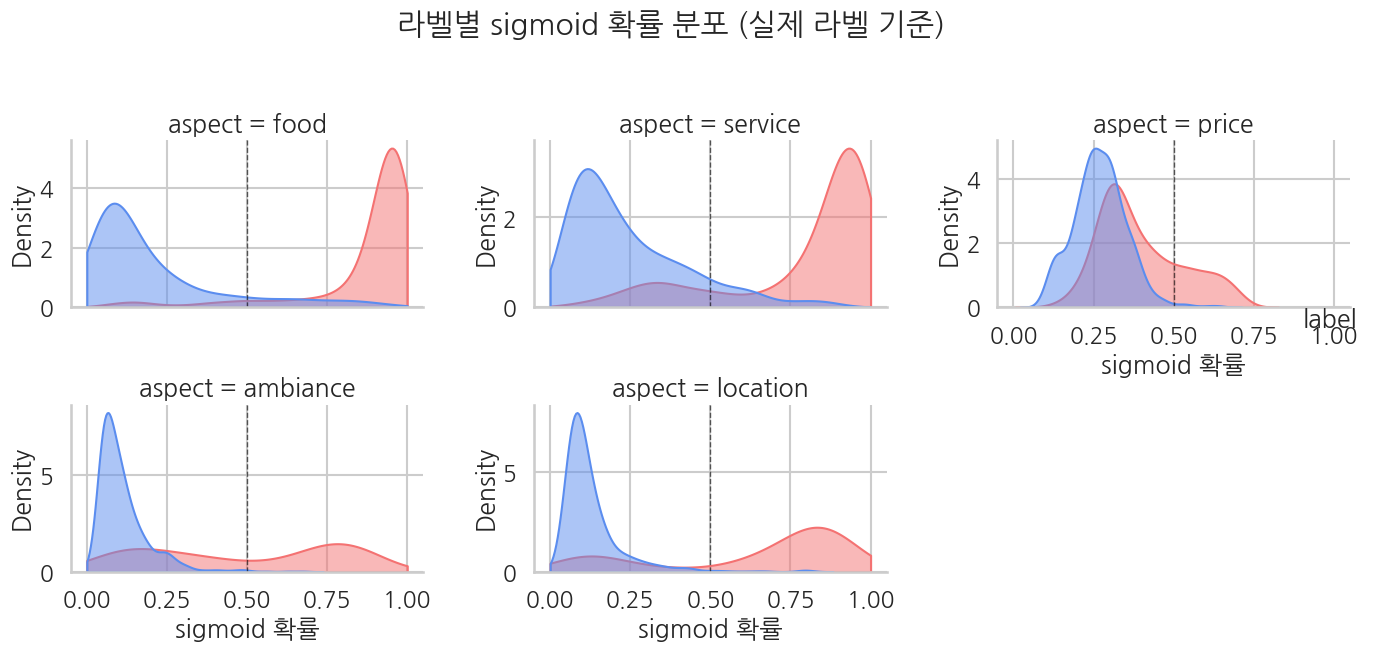
\includegraphics[width=0.94\linewidth]{assets/figures/ch13_label_probability_facets.png}
\end{bookfigurelabel}

\textbf{그림 읽기} --- 그림~\ref{fig:ch13-label-probability-facets}에서 다음 내용을 확인합니다: 라벨별 sigmoid 확률 분포. 실행된 노트북에서 저장된 최신 plot 출력이므로, 코드에서 계산한 값이 어떤 평가 지점으로 이어지는지 바로 확인할 수 있습니다.



\textbf{해석}

\begin{itemize}
\tightlist
\item
  \textbf{잘 학습된 라벨} (예: food): label=0 곡선은 0 근처, label=1 곡선은 1 근처에 있고 둘이 거의 만나지 않음. \emph{분리가 깨끗}.
\item
  \textbf{활성률이 낮은 라벨} (예: location): label=1 샘플이 적어 곡선이 노이즈가 큼. 그래도 분리는 보여야 함.
\item
  \textbf{두 곡선이 0.5 근처에서 크게 겹치면} \(\to\) 그 라벨은 모델이 잘 못 분리. 키워드 매칭이 \emph{얕아서} 진짜 신호를 못 잡았거나, 학습 데이터가 부족한 상태.
\end{itemize}



\subsection{라벨 공동 활성}

Multi-label 의 핵심 질문 중 하나: \emph{어떤 라벨 쌍이 같이 등장하는가?} 모델이 라벨 \emph{간 상관} 을 학습 데이터에서 흡수했는지 확인합니다.

\inlinecode{true\ co-occurrence} (실제 데이터의 라벨 동시 등장 빈도)와 \inlinecode{predicted\ co-occurrence} (모델 예측의 동시 등장 빈도)를 나란히 그려 두 행렬이 비슷하면 모델이 라벨 구조를 잘 잡고 있는 것.



\Needspace{11\baselineskip}
\begin{lstlisting}
def cooccurrence_matrix(Y):

    # Y: (N, K) multi-hot. Returns (K, K) where M[i,j] = P(label_j=1 | label_i=1).
    Y = Y.astype(float)
    K_ = Y.shape[1]
    M = np.zeros((K_, K_))
    for i in range(K_):
        row_i = Y[:, i]
        n_i = row_i.sum()
        if n_i == 0:
            continue
        for j in range(K_):
            M[i, j] = (row_i * Y[:, j]).sum() / n_i
    return M

\end{lstlisting}

\noindent\emph{앞 블록은 앞에서 만든 중간 값을 다음 계산으로 넘기는 단계입니다. 이어지는 블록에서는 숫자 결과를 그림으로 확인하는 단계로 넘어갑니다.}

\Needspace{11\baselineskip}
\begin{lstlisting}[firstnumber=16]
cooc_true = cooccurrence_matrix(labels)
cooc_pred = cooccurrence_matrix(preds)

fig, axes = plt.subplots(1, 2, figsize=(13, 5))
for ax, M, title in [
    (axes[0], cooc_true, "실제 동시출현  P(j | i)"),
    (axes[1], cooc_pred, "예측 동시출현  P(j | i)"),
]:
    sns.heatmap(
        M, annot=True, fmt=".2f", cmap="Blues", vmin=0, vmax=1,
        xticklabels=ASPECTS, yticklabels=ASPECTS,
        cbar_kws={"label": "조건부 확률"}, ax=ax,
    )
    ax.set_title(title)
    ax.set_xlabel("라벨 j")
    ax.set_ylabel("주어진 라벨 i")
\end{lstlisting}

\noindent\emph{앞뒤 블록은 모두 숫자 결과를 그림으로 확인하는 단계입니다. 길이를 나누어 같은 흐름을 단계별로 확인합니다.}

\Needspace{5\baselineskip}
\begin{lstlisting}[firstnumber=32]
plt.tight_layout()
plt.show()
\end{lstlisting}

\begin{bookfigurelabel}[H]{정답 라벨과 예측 라벨의 공동 활성 패턴}{fig:ch13-cooccurrence}
\centering
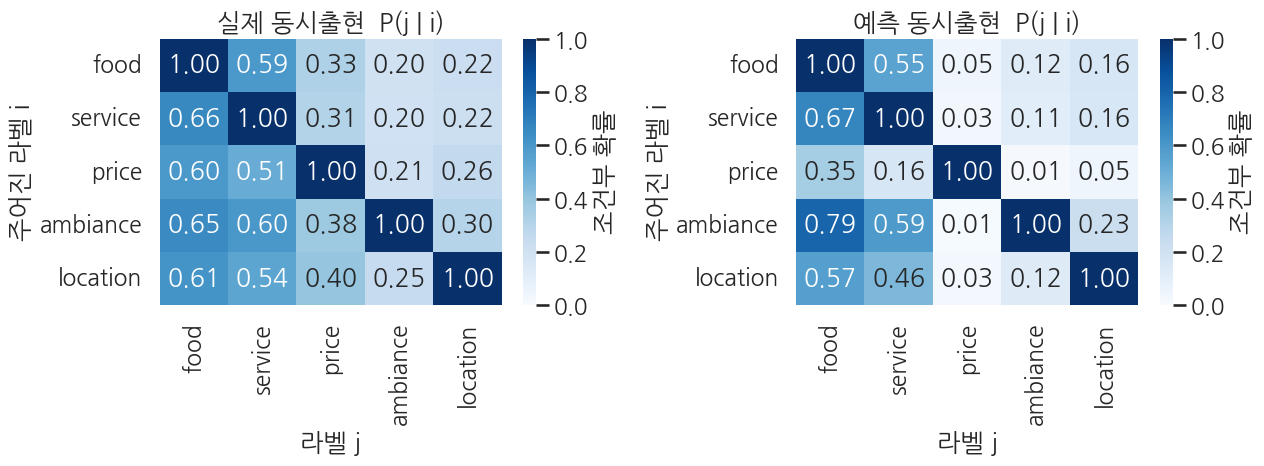
\includegraphics[width=0.96\linewidth]{assets/figures/ch13_cooccurrence.png}
\end{bookfigurelabel}

\textbf{그림 읽기} --- 그림~\ref{fig:ch13-cooccurrence}에서 다음 내용을 확인합니다: 정답 라벨과 예측 라벨의 공동 활성 패턴. 실행된 노트북에서 저장된 최신 plot 출력이므로, 코드에서 계산한 값이 어떤 평가 지점으로 이어지는지 바로 확인할 수 있습니다.



\textbf{해석}

\begin{itemize}
\tightlist
\item
  \textbf{대각선 = 1.0} --- 자기 자신과는 항상 같이 등장 (정의상).
\item
  \textbf{off-diagonal cell M{[}i, j{]}} = “라벨 i가 활성된 샘플 중 라벨 j 도 활성된 비율”. 비대칭 행렬.
\item
  food와 service가 같이 자주 등장하면 두 모델 모두 0.5+ 값. \emph{true} 와 \emph{predicted} 가 거의 비슷한 패턴이면 모델이 라벨 구조를 잘 학습했다는 뜻.
\item
  \textbf{predicted cell이 true cell 보다 일관되게 높으면} \(\to\) 모델이 라벨을 \emph{너무 많이} 활성하는 경향 (over-prediction). threshold를 0.5보다 높게 (예: 0.6) 두면 calibration 개선.
\end{itemize}



\section{\texorpdfstring{BERT와 sklearn 비교}{BERT와 sklearn 비교}}

\ref{ch:06}장의 sklearn 셋업을 \emph{이 노트북 안에서} 다시 학습해 라벨별로 BERT와 비교합니다. \textbf{multi-label에서도 BERT의 67M이 sklearn 대비 어디서 이기는가?}



\Needspace{11\baselineskip}
\begin{lstlisting}
texts_train = list(train_full["text"])
texts_eval  = list(eval_full["text"])
Y_train_bin = np.array(train_full["aspects"]).astype(int)
Y_eval_bin  = np.array(eval_full["aspects"]).astype(int)

vec = TfidfVectorizer(
    max_features=20000,
    ngram_range=(1, 2),
)
X_train = vec.fit_transform(texts_train)
X_eval  = vec.transform(texts_eval)

clf = OneVsRestClassifier(LogisticRegression(max_iter=2000, n_jobs=-1))
clf.fit(X_train, Y_train_bin)

\end{lstlisting}

\noindent\emph{앞 블록은 앞에서 만든 중간 값을 다음 계산으로 넘기는 단계입니다. 이어지는 블록에서는 예측 결과를 지표와 표로 요약하는 단계로 넘어갑니다.}

\Needspace{11\baselineskip}
\begin{lstlisting}[firstnumber=16]
probs_sk = clf.predict_proba(X_eval)        # (N, 5)
preds_sk = (probs_sk >= 0.5).astype(int)    # (N, 5)

p_mi_sk, r_mi_sk, f1_mi_sk, _ = precision_recall_fscore_support(
    Y_eval_bin, preds_sk, average="micro", zero_division=0,
)
p_ma_sk, r_ma_sk, f1_ma_sk, _ = precision_recall_fscore_support(
    Y_eval_bin, preds_sk, average="macro", zero_division=0,
)
auc_sk = float(roc_auc_score(Y_eval_bin, probs_sk, average="macro"))

\end{lstlisting}

\noindent\emph{앞 블록은 예측 결과를 지표와 표로 요약하는 단계입니다. 이어지는 블록에서는 앞에서 만든 중간 값을 다음 계산으로 넘기는 단계로 넘어갑니다.}

\Needspace{11\baselineskip}
\begin{lstlisting}[firstnumber=27]
print(f"sklearn TF-IDF + OvR LogReg:")
print(f"  vocabulary size:    {len(vec.vocabulary_):,}")
print(f"  micro F1:           {f1_mi_sk:.4f}")
print(f"  macro F1:           {f1_ma_sk:.4f}")
print(f"  macro AUC:          {auc_sk:.4f}")
print(
    f"  hamming loss:       "
    f"{hamming_loss(Y_eval_bin, preds_sk):.4f}"
)
\end{lstlisting}

\noindent\textbf{출력.}
\begin{bookoutputbox}
sklearn TF-IDF + OvR LogReg:
  vocabulary size:    20,000
  micro F1:           0.7634
  macro F1:           0.6141
  macro AUC:          0.9387
  hamming loss:       0.1426
\end{bookoutputbox}
\par\vspace{0.9em}



\subsection{평가지표 비교}



\Needspace{11\baselineskip}
\begin{lstlisting}
metrics_bert = {
    k.replace(
        "eval_",
        ""): v for k,
        v in eval_metrics.items(,
    )
    if k.startswith("eval_") and isinstance(v, float)
}
metrics_sk = {
    "hamming_loss":    float(hamming_loss(Y_eval_bin, preds_sk)),
    "micro_f1":        float(f1_mi_sk),
    "micro_precision": float(p_mi_sk),
    "micro_recall":    float(r_mi_sk),
    "macro_f1":        float(f1_ma_sk),
    "macro_precision": float(p_ma_sk),
    "macro_recall":    float(r_ma_sk),
\end{lstlisting}

\noindent\emph{앞뒤 블록은 모두 예측 결과를 지표와 표로 요약하는 단계입니다. 길이를 나누어 같은 흐름을 단계별로 확인합니다.}

\Needspace{11\baselineskip}
\begin{lstlisting}[firstnumber=17]
    "macro_auc":       auc_sk,
}

common = [k for k in metrics_bert if k in metrics_sk]
cmp = pd.DataFrame({
    "metric":             common,
    "sklearn (OvR)":      [metrics_sk[k]   for k in common],
    "BERT (this chapter)":[metrics_bert[k] for k in common],
})
cmp["BERT - sklearn"] = cmp["BERT (this chapter)"] - cmp["sklearn (OvR)"]
print(cmp.round(4).to_string(index=False))
\end{lstlisting}

\noindent\textbf{출력.}
\begin{bookoutputbox}
metric  sklearn (OvR)  BERT (this chapter)  BERT - sklearn
   hamming_loss         0.1426               0.1246         -0.0180
       micro_f1         0.7634               0.7977          0.0343
micro_precision         0.8915               0.9056          0.0141
   micro_recall         0.6674               0.7127          0.0453
       macro_f1         0.6141               0.7239          0.1099
macro_precision         0.9036               0.9155          0.0119
   macro_recall         0.5307               0.6447          0.1140
      macro_auc         0.9387               0.8994         -0.0393
\end{bookoutputbox}
\par\vspace{0.9em}



\subsection{라벨별 F1 비교}



\Needspace{11\baselineskip}
\begin{lstlisting}
def per_label_f1(Y_true, Y_pred):
    f1s = []
    for k in range(K):
        _, _, f1, _ = precision_recall_fscore_support(
            Y_true[:, k], Y_pred[:, k], average="binary", zero_division=0,
        )
        f1s.append(float(f1))
    return f1s

f1_bert = per_label_f1(labels, preds)
f1_sk   = per_label_f1(Y_eval_bin, preds_sk)

\end{lstlisting}

\noindent\emph{앞 블록은 예측 결과를 지표와 표로 요약하는 단계입니다. 이어지는 블록에서는 숫자 결과를 그림으로 확인하는 단계로 넘어갑니다.}

\Needspace{11\baselineskip}
\begin{lstlisting}[firstnumber=13]
label_cmp = pd.DataFrame({
    "aspect":     ASPECTS,
    "sklearn F1": f1_sk,
    "BERT F1":    f1_bert,
})
label_cmp["BERT - sklearn"] = label_cmp["BERT F1"] - label_cmp["sklearn F1"]
print(label_cmp.round(4).to_string(index=False))

fig, ax = plt.subplots(figsize=(10, 5))
x_pos = np.arange(K)
width = 0.38
\end{lstlisting}

\noindent\emph{앞 블록은 숫자 결과를 그림으로 확인하는 단계입니다. 이어지는 블록에서는 앞에서 만든 중간 값을 다음 계산으로 넘기는 단계로 넘어갑니다.}

\Needspace{11\baselineskip}
\begin{lstlisting}[firstnumber=24]
ax.bar(
    x_pos - width/2,
    f1_sk,
    width,
    label="sklearn (OvR)",
    color="#5B8DEF",
)
ax.bar(
    x_pos + width/2,
    f1_bert,
    width,
    label="BERT (이번 챕터)",
    color="#F47272",
)
ax.set_xticks(x_pos)
ax.set_xticklabels(ASPECTS)
\end{lstlisting}

\noindent\emph{앞 블록은 앞에서 만든 중간 값을 다음 계산으로 넘기는 단계입니다. 이어지는 블록에서는 숫자 결과를 그림으로 확인하는 단계로 넘어갑니다.}

\Needspace{8\baselineskip}
\begin{lstlisting}[firstnumber=40]
ax.set_ylim(0, 1)
ax.set_ylabel("라벨별 F1")
ax.set_title("라벨별 F1 — sklearn OvR vs BERT")
ax.legend()
plt.tight_layout()
plt.show()
\end{lstlisting}

\noindent\textbf{출력.}
\begin{bookoutputbox}
aspect  sklearn F1  BERT F1  BERT - sklearn
    food      0.9057   0.9203          0.0146
 service      0.8833   0.8545         -0.0288
   price      0.5271   0.3708         -0.1563
ambiance      0.3333   0.6510          0.3176
location      0.4211   0.8232          0.4022
\end{bookoutputbox}
\par\vspace{0.9em}

\begin{bookfigurelabel}[H]{라벨별 F1: sklearn OvR와 BERT 비교}{fig:ch13-f1-compare}
\centering
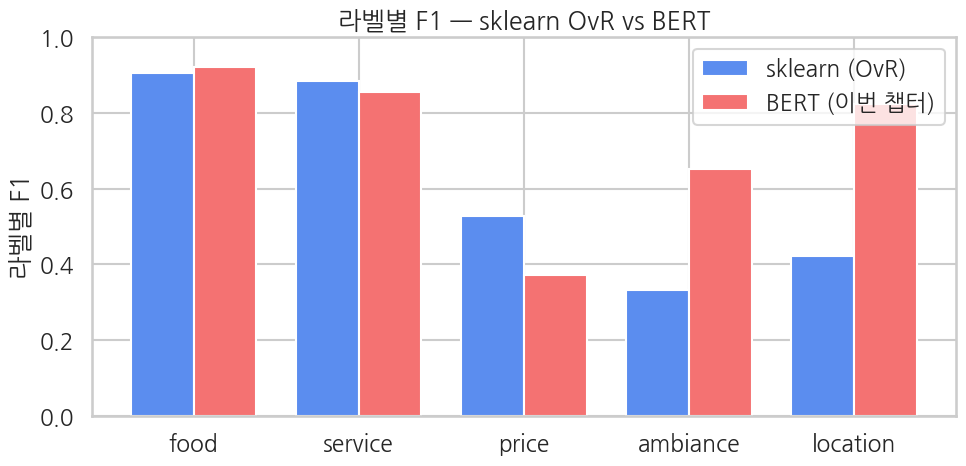
\includegraphics[width=0.88\linewidth]{assets/figures/ch13_f1_compare.png}
\end{bookfigurelabel}

\textbf{그림 읽기} --- 그림~\ref{fig:ch13-f1-compare}에서 다음 내용을 확인합니다: 라벨별 F1: sklearn OvR와 BERT 비교. 실행된 노트북에서 저장된 최신 plot 출력이므로, 코드에서 계산한 값이 어떤 평가 지점으로 이어지는지 바로 확인할 수 있습니다.



\textbf{해석}

\begin{itemize}
\tightlist
\item
  키워드 매칭으로 합성한 라벨은 \emph{키워드 단어가 본질 신호} 라 sklearn TF-IDF가 의외로 강합니다 --- 라벨 정의 자체가 단어 빈도와 일치하기 때문.
\item
  BERT가 \emph{큰 폭으로} 이기는 라벨이 있다면 \(\to\) 그 라벨의 \emph{합성 룰이 키워드만으로 안 잡히는 신호} 를 BERT가 추가로 학습한 것 (예: ambiance에서 “lighting was perfect” 같은 묘사).
\item
  BERT가 \emph{지는 라벨} 도 있을 수 있음 --- 키워드가 \emph{결정적} 인 라벨에서 sklearn은 \emph{완벽} 한 매칭, BERT는 \emph{근사} 라 약간의 noise가 들어감.
\end{itemize}

\textbf{합성 라벨의 본질적 한계} --- 이 비교는 \emph{키워드 매칭으로 만든 라벨} 위에서의 비교. 실제 사람-annotated multi-label 데이터에선 BERT 격차가 훨씬 큼 (단어 빈도로 안 잡히는 미묘한 항목 인식이 BERT의 강점).



\section{이 장에 등장한 라이브러리·함수}

\begin{booktable}{13장 새로 등장한 라이브러리}{tab:ch13-05}
\begin{adjustbox}{max width=\textwidth}
\begin{tabular}{@{}lll@{}}
\toprule
이름 & 한 줄 설명 & 다음 장에서 \\
\midrule

\inlinecode{AutoModelForSequenceClassification(num\_labels=5,\ problem\_type="multi\_label\_classification")} & \ref{ch:12}장 셋업에서 problem\_type만 변경 \(\to\) BCE per-label 자동 매핑 & \ref{ch:14}장에서 메인 헤드로 그대로 \\
\inlinecode{sklearn.metrics.hamming\_loss} & 전체 (sample \(\times\) label) 위치에서 틀린 비율 & multi-label 장마다 \\
\inlinecode{precision\_recall\_fscore\_support(...,\ average="micro"/"macro")} & multi-label용 F1 --- micro는 라벨 합산, macro는 라벨 평균 & \ref{ch:14}·\ref{ch:17}장·18 \\
\inlinecode{roc\_auc\_score(...,\ average="macro")} & 라벨별 AUC를 평균 & \ref{ch:17}·\ref{ch:18}장 \\
\inlinecode{seaborn.FacetGrid\ +\ map\_dataframe} & 5개 라벨에 같은 KDE를 facet으로 & 라벨이 많은 시각화에 재등장 \\
\inlinecode{OneVsRestClassifier(LogisticRegression())} & sklearn multi-label baseline & 비교용 \\
\bottomrule
\end{tabular}
\end{adjustbox}
\end{booktable}



\section{체크포인트 질문}

\begin{enumerate}
\def\labelenumi{\arabic{enumi}.}
\tightlist
\item
  multi-label 문제를 \emph{softmax + CrossEntropyLoss} 로 풀려고 하면 무엇이 잘못되나요? 수식으로 한 줄 설명할 수 있나요?
\item
  \inlinecode{num\_labels=5} 가 \ref{ch:12}장과 \ref{ch:13}장에서 \emph{같은 숫자} 인데 \emph{모델이 학습하는 의미} 는 어떻게 다른가요?
\item
  Macro F1과 Micro F1의 차이는 무엇이고, 어느 한쪽이 \emph{훨씬} 낮으면 무엇을 의심해야 하나요?
\item
  라벨별 \emph{공동 활성 행렬} 에서 모델 예측이 실제보다 일관되게 높은 행을 보였다면 어떤 처치가 필요한가요?
\end{enumerate}



\section{FAQ}

\begin{faqBox}{Q1. (실무) Multi-label에서 threshold 0.5는 항상 옳은가요?}

아닙니다. 0.5는 \emph{기본값} 일 뿐 라벨마다 최적 threshold가 다를 수 있습니다.

\begin{itemize}
\tightlist
\item
  \textbf{클래스 불균형}: 라벨 활성률이 5\% 인 라벨에선 0.5가 너무 보수적 --- 모델이 거의 안 활성. threshold를 0.2-0.3으로 낮추면 recall이 크게 올라감.
\item
  \textbf{F1 최적 threshold 탐색}: validation set에서 \emph{라벨별로} 0.1-0.9 grid search \(\to\) F1 최대 지점 선택.
\end{itemize}

\Needspace{11\baselineskip}
\begin{lstlisting}
def best_threshold(probs_k, labels_k):
    best_f1, best_th = 0, 0.5
    for th in np.arange(0.1, 0.91, 0.05):
        preds_k = (probs_k >= th).astype(int)
        _, _, f1, _ = precision_recall_fscore_support(
            labels_k,
            preds_k,
            average="binary",
            zero_division=0,
        )
        if f1 > best_f1:
            best_f1, best_th = f1, th
    return best_th, best_f1

thresholds = [best_threshold(probs[:, k], labels[:, k])[0] for k in range(K)]
\end{lstlisting}

운영 환경에선 \emph{라벨별 threshold} 를 저장해 두고 추론 시 적용.

\end{faqBox}

\begin{faqBox}{Q2. (이론) Multi-class를 multi-label로 풀어도 되나요? (single-label 데이터를 multi-hot 형식으로 변환)}

기술적으론 됩니다. 단점이 큽니다.

\begin{booktable}{13장 FAQ 표}{tab:ch13-06}
\begin{adjustbox}{max width=\textwidth}
\begin{tabular}{@{}lll@{}}
\toprule
& multi-class (CE) & single-label을 multi-label (BCE) 로 \\
\midrule

라벨 간 \emph{경쟁} 학습 & softmax가 자동으로 강제 & BCE per-label은 라벨 간 직접 신호 없음 \\
confidence 의미 & 항상 합 = 1, 명확 & 5개 라벨의 sigmoid 확률, \emph{합 \(\ne\) 1} \\
추론 후처리 & \inlinecode{argmax} 한 줄 & \inlinecode{argmax(probs)} 또는 \texttt{np.where(probs\ \textgreater{}\ th)} \\
학습 수렴 속도 & 빠름 (라벨 경쟁 신호 있음) & 약간 느림 \\
\bottomrule
\end{tabular}
\end{adjustbox}
\end{booktable}

multi-class가 \emph{명확히 single-label} 이면 CE가 정답. multi-label로 푸는 건 \emph{어떤 이유로 두 task를 통합해야 할 때} (예: \ref{ch:14}장 보조 헤드처럼).

\end{faqBox}

\begin{faqBox}{Q3. (실무) Class weights를 multi-label BCE에 적용하려면?}

\inlinecode{pos\_weight} 파라미터 --- \inlinecode{BCEWithLogitsLoss(pos\_weight=...)} 가 라벨별 양성 가중치를 받습니다.

\Needspace{9\baselineskip}
\begin{lstlisting}
import torch
from torch import nn

pos_count = Y_train_bin.sum(axis=0)
neg_count = len(Y_train_bin) - pos_count
pos_weight = torch.tensor(neg_count / np.maximum(pos_count, 1), dtype=torch.float).to("cuda")
loss_fn = nn.BCEWithLogitsLoss(pos_weight=pos_weight)
\end{lstlisting}

\inlinecode{Trainer.compute\_loss} 를 오버라이드해서 위 \inlinecode{loss\_fn} 으로 바꾸면 됩니다. 활성률 5\%인 라벨은 pos\_weight \(\approx\) 19 \(\to\) 양성 샘플의 손실이 19배 가중되어 모델이 양성 예측을 더 자주 하도록 강제.

\end{faqBox}

\begin{faqBox}{Q4. (이론) 모델이 라벨 \emph{간} 상관을 학습하는 메커니즘은? (loss엔 라벨 결합 항이 없는데)}

핵심은 \textbf{공유 BERT 본체} 입니다. 5개 라벨의 logit이 같은 768-dim CLS hidden state \(h\) 에서 \emph{별도의 5개 가중치 행} 을 통해 나옵니다.

\begin{equation}
\label{eq:ch13-02}
z_k = w_k^\top h + b_k, \quad k = 1, \ldots, K
\end{equation}

식~\eqref{eq:ch13-02}은 이 절에서 사용하는 핵심 관계를 정리한 것입니다.

학습 중:

\begin{itemize}
\tightlist
\item
  라벨 1이 활성된 샘플에서 \(w_1\) 이 \(h\) 의 특정 차원을 강조하도록 학습됩니다.
\item
  같은 샘플에서 라벨 2도 활성됐다면 \(w_2\) 도 \emph{비슷한 차원} 을 강조하게 됩니다.
\item
  결과적으로 라벨 1과 2가 같이 활성되는 \emph{입력 패턴} 에 대해 두 logit이 동시에 커지는 \emph{간접} 결합이 생깁니다.
\end{itemize}

Loss에는 결합 항이 없지만 \emph{gradient가 BERT 본체를 거쳐 흐를 때} 결합이 자연스럽게 학습됩니다. 이게 BERT 같은 \emph{공유 표현} 모델이 multi-label에서 sklearn OvR 보다 강한 이유 --- sklearn은 K개 LogReg가 \emph{완전 분리} 학습되므로 이런 간접 결합이 없습니다.

\end{faqBox}

\begin{faqBox}{Q5. (실무) 라벨이 100개 이상인 multi-label은 BERT로 어떻게 푸나요?}

\textbf{일반적 패턴}:

\begin{enumerate}
\def\labelenumi{\arabic{enumi}.}
\tightlist
\item
  \textbf{라벨이 \textasciitilde50개 이하}: \inlinecode{num\_labels=K} + per-label sigmoid + BCE 그대로. 본 장 패턴.
\item
  \textbf{라벨이 100-1000개}: 헤드의 weight matrix가 커짐 (768·K). 메모리 압박. 해결책:

  \begin{itemize}
  \tightlist
  \item
    \textbf{Hierarchical labels}: 라벨을 트리로 구조화해 \emph{상위 \(\to\) 하위} 단계적 분류 (예: “음식 \textgreater{} 한식 \textgreater{} 김치찌개”)
  \item
    \textbf{Knowledge distillation}: 큰 multi-label 모델에서 작은 모델로 distill
  \end{itemize}
\item
  \textbf{라벨이 1000+ 개}: extreme multi-label (XML). 별도 분야 --- \inlinecode{XML-CNN}, \inlinecode{BERT-XMC} 등 특화 모델 사용.
\end{enumerate}

영화 장르 분류 (\textasciitilde30개), 기사 토픽 (\textasciitilde50개) 정도면 본 장 패턴으로 충분.

\end{faqBox}

\begin{faqBox}{Q6. (실무) Multi-label에서 \emph{클래스가 추가되면} 모델을 처음부터 다시 학습해야 하나요?}

기본적으론 그렇습니다. 분류 헤드의 weight shape이 \inlinecode{(K,\ 768)} 이라 K가 바뀌면 헤드가 호환 안 됨. 단, BERT 본체는 그대로 재사용 가능.

\Needspace{9\baselineskip}
\begin{lstlisting}
old_model = AutoModelForSequenceClassification.from_pretrained("./ch13_output")
new_model = AutoModelForSequenceClassification.from_pretrained(
    "distilbert-base-uncased", num_labels=6, problem_type="multi_label_classification",
)

new_model.classifier.weight.data[:5] = old_model.classifier.weight.data
new_model.classifier.bias.data[:5]   = old_model.classifier.bias.data
\end{lstlisting}

이러면 기존 5라벨은 \emph{학습된 상태로 시작}, 6번째만 \emph{처음부터 학습} . 실무에서 자주 쓰는 incremental learning 패턴.
\end{faqBox}



\section{오류 실험 (선택)}

다음 코드를 돌려보면 어떤 에러가 날까요?

\Needspace{11\baselineskip}
\begin{lstlisting}
def tokenize_wrong(batch):
    out = tokenizer(
        batch["text"],
        truncation=True,
        max_length=128,
    )

    out["labels"] = [
        next((i for i, v in enumerate(a) if v > 0), 0)
        for a in batch["aspects"]
    ]
    return out
\end{lstlisting}

힌트: \inlinecode{BCEWithLogitsLoss} 는 \emph{logits 와 같은 shape의 float 텐서} 를 라벨로 받는데, 위 코드는 \emph{(B,) int} 를 넘깁니다. shape mismatch + dtype mismatch 두 가지 에러가 동시에 날 수 있어 메시지가 길어집니다.



\begin{previewBox}{미리보기: 다음 장}

\textbf{\ref{ch:14}장. BERT Auxiliary Loss --- 항목 분류 + 별점 보조 회귀}

\begin{itemize}
\tightlist
\item
  메인 task: \ref{ch:13}장의 multi-label 항목 분류 (\inlinecode{num\_labels=5} + BCE per-label) --- \emph{완전히 동일}
\item
  추가: \emph{보조 헤드} \inlinecode{Linear(H,\ 1)} 로 별점 점수 회귀 (별점 정규화 0-1)
\item
  손실: \texttt{L\ =\ BCE\_per\_label(메인)\ +\ \$\textbackslash{}lambda\$\ ·\ MSE(보조)} 가중합 (\(\lambda\)는 hyperparameter)
\item
  \inlinecode{Trainer.compute\_loss} 오버라이드로 두 헤드를 동시 학습
\item
  보조 task가 메인 task의 정확도를 \emph{얼마나 끌어올리는지} 측정 (auxiliary loss의 정통 활용)
\end{itemize}

\begin{quote}
\textbf{변하는 축}: 메인 task와 모델 본체는 그대로, \emph{Loss에 보조 항이 추가} 됩니다 --- Loss 축의 마지막 단계 (“BCE per-label \(\to\) +Auxiliary”).
\end{quote}
\end{previewBox}